% Remove number from chapter
\makeatletter
\titleformat{\chapter}%
  [display]% shape
  {\relax\ifthenelse{\NOT\boolean{@tufte@symmetric}}{\begin{fullwidth}}{}}% format applied to label+text
%  {\itshape\huge\thechapter}% label
  {}% label
  {0pt}% horizontal separation between label and title body
  {\huge\rmfamily\itshape}%\thechapter. }% before the title body
  [\ifthenelse{\NOT\boolean{@tufte@symmetric}}{\end{fullwidth}}{}]% after the title body
\makeatother


\chapter*{Ответы}
\markboth{Ответы}{} % remove "Chapter" numbering in headline (top right)
\label{ch:answers}
\addcontentsline{toc}{chapter}{Ответы}% add line to toc but without the number of chapter
	
\setcounter{footnote}{0}% restart footnotes

%\TODO uncomment
%\epigraph{%
%Ставлю три звездочки. 
%Я видал в детских книжках: 
%когда человек делает прыжок к новой мысли, 
%он~ставит три звездочки\ldots%
%}{%
%Саша Чёрный. Дневник Фокса Микки}


В каждой из глав на полях даются задания, а ответы на них собраны здесь.
\marginnote[-3\baselineskip]{
    \MarginQuestion
    Таким значком-лампочкой отмечены на полях вопросы. 
    Не~на~все из~них, но~на~большинство ответы представлены ниже.
}

\begin{task}
    \label{answer:instance-in-OOP-vs-Wikidata}
    \AnswerBackref Вопрос на с.~\pageref{question:instance-in-OOP-vs-Wikidata}.

    Экземпляр объекта\footnote[][0cm]{%
        См. статью 
        \href{https://en.wikipedia.org/wiki/Instance\_(computer\_science)}{Instance (computer science)} в Английской Википедии.
%
    } в Викиданных 
    и в объектно-ориентированном программировании (ООП) сходны в сути, а именно:
    есть модель базового объекта $D$, создаётся новая единица $I$, обладающая 
    свойствами той же модели $D$. 
    В программировании о создании $I$ говорят, 
    что класс $D$ проинициализирован 
    и получен объект $I$\footnote[][0cm]{%
        $I$~является экземпляром $D$, или 
        \mbox{$I$~is instance of $D$}~--- по-английски.}. 
%        $I$~is instance of $D$ по-английски, 
%        $I$~является экземпляром $D$ \mbox{по-русски}}.

    В чём разница? 
    В ООП в исходном коде программы мы видим, как во времени последовательно 
    (в~разных строках программы) происходит 
    объявление переменной, инициализация класса, 
    присвоение значений экземплярам класса.
    В Викиданных в тот момент, когда выполняется скрипт и происходит обращение 
    к данным, объекты, являющиеся экземплярами других объектов, 
    уже представлены и обычно не происходит их изменение, 
    связанное с~работой SPARQL-скриптов.
\end{task}



%%%%%%%%%%%%%% Aircraft chapter %%%%%%%%%%%%%%
\marginnote[1\baselineskip]{%
    \pgfornament[width=1.2cm]{80}%

    \noindent Таким орнаментом мы разделим ответы на~вопросы из разных глав.%
}
\hfil\pgfornament[width=4cm]{80}\hfil%



\newpage
\begin{task}
    \label{answer:aircraft_manufacturers}
    \AnswerBackref Вопрос на с.~\pageref{lst:lang2}.

    Веб-сайты есть у следующих российских производителей: 
    <<МиГ>>, <<Туполев>> и <<Сухой>>. 
    Эти сайты можно получить с~помощью запроса~\ref{lst:aircraft_manufactures_lst}. 

\begin{lstlisting}[ 
            language=SPARQL, 
            caption={\href{https://w.wiki/t4H}{Веб-сайты российских авиазаводов}\protect\footnotemark}, 
            label=lst:aircraft_manufactures_lst, 
            numbers=none,
            ]
SELECT ?manufacturer ?manufacturerLabel ?site WHERE
{
  ?manufacturer wdt:P31 wd:Q936518. # instance of aerospace manufacturer
  ?manufacturer wdt:P17 wd:Q159. # country Russia
  ?manufacturer wdt:P856 ?site # official website
  SERVICE wikibase:label {bd:serviceParam wikibase:language "ru"}
}
\end{lstlisting}
\footnotetext{Получено: 14 авиазаводов в России с веб-сайтами на 2020 год. Ссылка на SPARQL-запрос: \href{https://w.wiki/t4H}{https://w.wiki/t4H}.}
\end{task}


\begin{task}
    \label{answer:aircraft_company_foundation_date}
    \AnswerBackref Вопрос на с.~\pageref{aircraft_question_2}.
    
    Компания 
<<Туполев>> была основана в 1922 году, 
<<МиГ>> и <<Сухой>>~--- в 1939-м, 
<<Вымпел>>~--- в 1949 году.
    Ответ на~вопрос можно получить, выполнив запрос~\ref{lst:aircraft_company_foundation_date_lst}. 
    
	\begin{lstlisting}[ 
            language=SPARQL, 
            caption={\href{https://w.wiki/vaH}{Даты основания отечественных авиазаводов}\protect\footnotemark}, 
            label=lst:aircraft_company_foundation_date_lst, 
            numbers=none,
            ]
# Russian aircraft factories sorted by inception years
SELECT ?manufacturer ?manufacturerLabel (YEAR(?inception) AS ?year) WHERE 
{
  ?manufacturer wdt:P31 wd:Q936518;  # is aerospace manufacturer
                wdt:P17 wd:Q159;     # country Russia
                wdt:P571 ?inception. # foundation date
  SERVICE wikibase:label {bd:serviceParam wikibase:language "ru"}
}
ORDER BY ?year
\end{lstlisting}
\footnotetext{Получено: 15 отечественных авиазаводов с датой основания на 2021 год. Ссылка на SPARQL-запрос: \href{https://w.wiki/vaH}{https://w.wiki/vaH}.}
\end{task}


\begin{task}
    \label{answer:aircraft_company_headquarters}
    \AnswerBackref Вопрос на с.~\pageref{aircraft_question_3}.

Штаб-квартира компании <<Камов>> находится в городе Люберцы, 
    <<Авиадвигатель>>~--- в~Перми, 
    <<Улан-Удэнский авиационный завод>>~--- в городе Улан-Удэ, 
    <<Сухой>>~--- в Москве. 
    Ответ на~вопрос можно получить, выполнив запрос~\ref{lst:aircraft_company_headquarters_lst}. 
   

\newpage
\begin{lstlisting}[ 
            language=SPARQL, 
            caption={\href{https://w.wiki/t4X}{Штаб-квартиры компаний}\protect\footnotemark}, 
            label=lst:aircraft_company_headquarters_lst, 
            numbers=none,
                    ]
SELECT ?manufacturer ?manufacturerLabel ?inceptionLabel WHERE
{
    ?manufacturer wdt:P31 wd:Q936518. # instance of aerospace manufacturer
  	?manufacturer wdt:P17 wd:Q159. # country Russia
  	?manufacturer wdt:P159 ?inception # headquarters location
    SERVICE wikibase:label {bd:serviceParam wikibase:language "ru"}
}
\end{lstlisting}
\footnotetext{Получено: 16 российских авиазаводов, имеющих штаб-квартиры в~2021~году.\, Ссылка на SPARQL-запрос: \href{https://w.wiki/t4X}{https://w.wiki/t4X}.}
\end{task}


\begin{task}
    \label{answer:aircraft_question_airship}
    \AnswerBackref Вопрос на с.~\pageref{aircraft_question_4}.

Воздушным судном, удерживаемым в воздухе огромным баллоном 
    с горючим и смертельно опасным газом, 
    расположенным прямо над головами пассажиров, является дирижабль. 
\end{task}



% Unknown old Soviet airship on black and white photo
%
\begin{task}
    \label{answer:aircraft_question_airship_2}
    \AnswerBackref Вопрос на с.~\pageref{fig:airship_question_aircraft}.

Воздушное судно, 
    изображенное на~с.~\pageref{fig:airship_question_aircraft},~--- 
    это дирижабль \ruwiki{wKY}{СССР--В6 <<Осоавиахим>>} (1934--1938), 
    который установил мировой рекорд в~1937 году, 
    пролетев 130 с~половиной часов без посадки.
    Для~построения <<плиточки>> (ImageGrid) из иллюстраций дирижаблей 
    выполните запрос~\ref{lst:aircraft_airship_photo_lst}.
    
	\begin{lstlisting}[ 
            language=SPARQL, 
            caption={\href{https://w.wiki/t4c}{Изображения дирижаблей}\protect\footnotemark}, 
            label=lst:aircraft_airship_photo_lst, 
            numbers=none,
                    ]
#defaultView:ImageGrid
SELECT ?airship ?airshipLabel ?image WHERE
{
    ?airship wdt:P31 wd:Q133585. # instance of airship
  	?airship wdt:P18 ?image # image airship
    SERVICE wikibase:label {bd:serviceParam wikibase:language "ru"}
}
\end{lstlisting}
\footnotetext{Получено: 18 дирижаблей с иллюстрациями в~2021~году. Ссылка на~SPARQL-запрос: \href{https://w.wiki/t4c}{https://w.wiki/t4c}.}
\end{task}
%eo Aircraft chapter %%%%%%%%%%%%%%%%%%%%%%%%%%%%%%%%
%%%%%%%%%%%%%%%%%%%%%%%%%%%%%%%%%%%%%%%%%%%%%%%%%%%%%



%%%%%%%%%%%%%% Anime charpter %%%%%%%%%%%%%%
%eo Anime chapter %%%%%%%%%%%%%%%%%%%%%%%%%%%%%%%%




\hfil\pgfornament[width=4cm]{80}\hfil%
\newpage
%%%%%%%%%%%%%%% Human_settlements charpter %%%%%%%%%%

\begin{task}
\label{answer:human_settlements_density}
    \AnswerBackref Вопрос на с.~\pageref{ch:human-settlement}.

    Плотность населения в Алейске составляет 648 чел./км\textsuperscript{2}, 
        в~Барабинске~--- 413 чел./км\textsuperscript{2}, 
        то есть в~Алейске плотность выше. 

        Плотность населения по населённым пунктам России можно получить 
        с~помощью запроса~\ref{lst:human_settlements_density}. 

        Обратите внимание, что площадь может быть задана в разных единицах. 
        Например, у~\wdqName{Алейска}{11304591} площадь в Викиданных указана в гектарах, 
        у~\wdqName{Барабинска}{104609}~--- в квадратных километрах. 
        Для нормализации данных и перевода площади в~метры в~строке~8 запроса~\ref{lst:human_settlements_density}
        указан префикс \lstinline|psn:|. 

        В~строке~2 делим \lstinline|?area| на миллион, чтобы перевести квадратные метры в километры. 
        Результат деления записываем в~переменную \lstinline|?popArea|, которая показывает плотность населения. 


\index{SPARQL!psn:!нормализация площади}
\begin{lstlisting}[ language=SPARQL, 
                    caption={\href{https://w.wiki/6ibN}{Плотность населения <<населенных пунктов>> России}\protect\footnotemark},
                    label=lst:human_settlements_density,
                    xleftmargin=18pt, 
                  ]
# population density of human settlements in Russia
SELECT ?hum ?humLabel ?population ?area (?population / (?area / 1000000) as ?popArea) 
WHERE {
    ?hum wdt:P31 wd:Q486972; # is human settlement
         wdt:P17 wd:Q159;    # in Russia
       
    # The psn: prefix normalizes the values to a common unit of area
    p:P2046/psn:P2046/wikibase:quantityAmount ?area;  # get the area
       
    wdt:P1082 ?population. # has ?population
    FILTER(?population>0 && ?area).
    SERVICE wikibase:label{bd:serviceParam wikibase:language "ru,en"}
}
ORDER BY DESC (?popArea)
\end{lstlisting}
\footnotetext{Получено: 131 населённый пункт в~России с~известной плотностью населения на~2021 год, 
                        152 пункта на~2023 год. 
              SPARQL-запрос: \href{https://w.wiki/6ibN}{https://w.wiki/6ibN}.}
\end{task}



\begin{task}
\label{answer:flag_human_settlements}
    \AnswerBackref
    Вопросы на с.~\pageref{fig:flag_question_human_settlements1}, \pageref{fig:flag_question_human_settlements2}, \pageref{fig:flag_question_human_settlements3}, \pageref{fig:flag_question_human_settlements4}, \pageref{fig:flag_question_human_settlements5}.

Гербы, изображенные на с.~\pageref{fig:flag_question_human_settlements1}, 
    \pageref{fig:flag_question_human_settlements2} и 
    \pageref{fig:flag_question_human_settlements5}, 
    являются гербами отечественных населённых пунктов. 
    Герб~на~с.~\pageref{fig:flag_question_human_settlements3} 
    принадлежит \ruwiki{4dUc}{чешскому} населённому пункту, 
    герб~на~с.~\pageref{fig:flag_question_human_settlements4}~--- 
    \ruwiki{4dUf}{украинскому}. 

Ответ можно получить с~помощью запроса~\ref{lst:flag_question_human_settlements}. 
    Значение свойства \wdProperty{94}{coat of arms image} 
    содержит изображение герба населённого пункта.

\newpage
\index{График!ImageGrid}
\begin{lstlisting}[ language=SPARQL, 
                    caption={\href{https://w.wiki/4e8A}{Гербы населённых пунктов Российской Федерации}\protect\footnotemark},
                    label=lst:flag_question_human_settlements,
                    numbers=none,
                  ]
# Emblems of human settlements in Russia
#defaultView:ImageGrid
SELECT ?hum ?humLabel ?image WHERE {
  ?hum wdt:P31 wd:Q486972; # instance of human settlement
       wdt:P17 wd:Q159;    # in Russia
       wdt:P94 ?image.     # coat of arms
  SERVICE wikibase:label{bd:serviceParam wikibase:language "ru, en"}
}
\end{lstlisting}
\footnotetext{Получено: 148 гербов на 2022 год. SPARQL-запрос: \href{https://w.wiki/4e8A}{https://w.wiki/4e8A}.}
\end{task}
% eo Human_settlements charpter %%%%%%%%%%%%%%%%%%%%%%




\hfil\pgfornament[width=4cm]{80}\hfil%
%%%%%%%%%%%%%% City chapter %%%%%%%%%%%%%%
\begin{task}
    \label{answer:cities_geographic_objects}
    \AnswerBackref Вопрос на с.~\pageref{lst:population_town}.

    В честь географических объектов были названы 
    Тула (\href{https://w.wiki/oLJ}{река Тулица}), 
    Курильск (\href{https://w.wiki/oLH}{Курильские острова}) 
    и Вологда (\href{https://w.wiki/oLG}{река Вологда}). 
    Ответ на~вопрос можно получить, выполнив запрос~\ref{lst:cities_geographic_objects}. 
    Значение свойства \wdProperty{138}{named after} 
    показывает, в честь какого объекта Викиданных был назван город.

\lstset{escapeinside={(*@}{@*)}}
\sethlcolor{pink}
%
\index{SPARQL!FILTER}
\index{SPARQL!Поиск подклассов!wdt:P31/wdt:P279*}
\begin{lstlisting}[ language=SPARQL, 
                    caption={\href{https://w.wiki/6icv}{Города, названные в честь географических объектов}\protect\footnotemark},
                    label=lst:cities_geographic_objects,
                    xleftmargin=18pt, 
                    ]
SELECT DISTINCT ?city ?cityLabel ?namedAfter ?namedAfterLabel 
WHERE {
  ?city wdt:P31/wdt:P279* (*@\hl{wd:Q7930989}@*). # instances/subclasses of "city/town" 
  ?city wdt:P138 ?namedAfter.          # with filled property "named after"
  FILTER(?city = wd:Q1341 || ?city = wd:Q156046 ||
         ?city = wd:Q2770 || ?city = wd:Q1957 ||
         ?city = wd:Q5655 || ?city = wd:Q175651)
  SERVICE wikibase:label { bd:serviceParam wikibase:language "ru" }
}
\end{lstlisting}%
\marginnote[-4.4cm]{
    $\twemoji[width=24pt]{cityscape}$\,\,
    В строке 3 запроса~\ref{lst:cities_geographic_objects} 
    после конструкции \lstinline|wdt:P31/wdt:P279*| следует объект Викиданных, 
    объединяющий \wdqName{city}{515} и \wdqName{town}{3957} 
    и называющийся \hl{{\wdqName{city/town}{7930989}}}. 
%                         \wdqName{city/town}{7930989}. 
    Такой поиск с~помощью подклассов позволяет найти экземпляры сразу обоих типов городов. 
    Подробности см. в~главе~<<\nameref{sect:city-completness}>>, 
    в~тексте, предшествующем запросу~\ref{lst:example_subclasses_city} на~с.~\pageref{lst:example_subclasses_city}.
    }
\footnotetext{Для 6 городов, заданных в строках 5--7, 
              получено 6 объектов, в честь которых названы города. 
              Из них 3 города названы в честь географических объектов (см.~выше), 
              2~--- в честь известных людей и 
              1~город~--- в честь железнодорожной станции. 
              Ссылка на SPARQL-запрос: \href{https://w.wiki/6icv}{https://w.wiki/6icv}.}
\end{task}



\begin{task}
    \label{answer:cities_over_400_age}
    \AnswerBackref Вопрос на с.~\pageref{fig:city_relation_Russia_S_N}.

    Более 400 лет назад были основаны Казань (1005 год), Москва (1147), 
    Астрахань (1558), Воронеж (1586) и Самара (1586). 
    Самым молодым городом оказался Саров, основанный в~1691 году. 
    Ответ на~вопрос можно получить, выполнив запрос~\ref{lst:cities_over_400_age}. 

   
    \newpage
    \index{SPARQL!FILTER!OR}
    \index{SPARQL!YEAR}
    \begin{lstlisting}[ language=SPARQL, 
                    caption={\href{https://w.wiki/6idC}{Города, основанные более 400 лет назад в России}\protect\footnotemark},
                    label=lst:cities_over_400_age,
                    xleftmargin=18pt, 
                    ]
SELECT ?city ?cityLabel (YEAR(?inceptionDate) AS ?year) 
WHERE {
    ?city wdt:P31/wdt:P279* wd:Q7930989. # instances of "city/town" subclasses
    ?city wdt:P17 wd:Q159.               # in Russia
    ?city wdt:P571 ?inceptionDate.       # with filled property "inception"  
    FILTER (YEAR(?inceptionDate) < 1620). # 2020 - 400 years
    FILTER(?city = wd:Q649 || ?city = wd:Q193522 || ?city = wd:Q900 ||
           ?city = wd:Q3927 || ?city = wd:Q894 || ?city = wd:Q3426)
  	SERVICE wikibase:label { bd:serviceParam wikibase:language "ru" }
}
GROUP BY ?city ?cityLabel ?inceptionDate
ORDER BY ASC(?year)
\end{lstlisting}
\footnotetext{Из 6 городов, заданных в строках 7--8, 
              получено 4 города в России, основанные до~1620 года. 
              Ссылка на SPARQL-запрос: \href{https://w.wiki/6idC}{https://w.wiki/6idC}.%
} 

Подумайте, какие строки в~запросе~\ref{lst:cities_over_400_age} нужно закомментировать, 
    чтобы получить, во-первых, список всех отечественных городов, 
    во-вторых, 
    список городов всего мира, основанных более 400 лет назад. 

Как вы думаете, может ли в запросе~\ref{lst:cities_over_400_age} 
    переменная \lstinline|?year| принимать отрицательные значения? 
    Если <<да>>, то почему?

    \index{SPARQL!Unknown value}
    Обычно значение свойства 
    \wdProperty{571}{inception} 
    содержит дату%
\sidenote{%
О типах данных и наборах свойств, связанных с датой и временем, 
    см.~справку на~странице Викиданных \href{https://w.wiki/NdT}{Help:Dates}.%
%
} основания города. 
Однако у~объекта Викиданных \wdqName{Москва}{649} 
    свойство inception 
    принимает значение unknown value (неизвестное значение) 
    с квалификатором <<самое позднее упоминание>> 
    (\wdProperty{1326}{latest date}), равным 4~апреля 1147 года. 
    Вероятно, по этой причине в~запросе~\ref{lst:cities_over_400_age} 
    переменная \lstinline|?year| принимает для~Москвы пустое значение, 
    и Москва ошибочно не попадает в список правильных ответов. 
    Таким образом, чтобы извлечь 1147 год, 
    необходимо доработать имеющийся скрипт, что мы и предоставим читателю. 
\end{task}


\begin{task}
    \label{answer:cities_flags}
    \AnswerBackref Вопрос на с.~\pageref{lst:countries_sister_cities_with_Russia}.

    Флаг, изображенный на рисунке, 
    принадлежит городу \href{https://ru.wikipedia.org/?curid=92075}{Карабулак}. 
    Ответ на~вопрос можно получить с~помощью запроса~\ref{lst:cities_flags}. 
    Значение свойства \wdProperty{41}{flag image} 
    содержит изображение флага города.
    
    \newpage
    \index{SPARQL!Поиск подклассов!wdt:P31/wdt:P279*}
    \begin{lstlisting}[ language=SPARQL, 
                    caption={\href{https://w.wiki/8orr}{Флаги городов России}\protect\footnotemark},
                    label=lst:cities_flags,
                    numbers=none,
                    ]
#defaultView:ImageGrid
SELECT ?city ?cityLabel ?flag ?countryLabel WHERE {
    ?city wdt:P31/wdt:P279* wd:Q7930989; # instances/subclasses of "city/town"
          wdt:P17 wd:Q159;               # in Russia
          wdt:P41 ?flag.                 # with filled property "flag"
    SERVICE wikibase:label { bd:serviceParam wikibase:language "ru" }
}
\end{lstlisting}
\footnotetext{Получено: 980 городов России имеют флаги на 2023 год. 
              Ссылка на~SPARQL-запрос: \href{https://w.wiki/8orr}{https://w.wiki/8orr}.}
\end{task}




\hfil\pgfornament[width=4cm]{80}\hfil%
%%%%%%%%%%%%%% Country chapter %%%%%%%%%%%%%%
\begin{task}
	\label{answer:administrative_territorial}
    \AnswerBackref Вопрос на с.~\pageref{lst:age_of_country}.

Речь идёт о количестве 
административно-территориальных единиц в~каждой из~стран, например: штаты, края или области. 
		%Количество административно-территориальных единиц у \href{https://w.wiki/mzN}{Латвии}  119, у \href{https://w.wiki/mzP}{Таиланда} 77, у \href{https://w.wiki/mzR}{Дании} 5, а у \href{https://w.wiki/myt}{России} 81. 
Количество таких единиц по~странам 
    можно получить с~помощью запроса~\ref{lst:administrative_territorial_entity}.
	
\begin{lstlisting}[ language=SPARQL, 
	caption={\href{https://w.wiki/8ory}{
	Список стран, упорядоченных по количеству административно-территориальных единиц}\protect\footnotemark},
	label=lst:administrative_territorial_entity,
    numbers=none,
    ]
# Countries sorted by number of administrative territories
SELECT ?country ?countryLabel  (count(*) as ?count) WHERE
{
    ?country p:P31 [ps:P31 wd:Q6256]; # is a country
             wdt:P150 [].         # has some administrative territory
    SERVICE wikibase:label { bd:serviceParam wikibase:language "ru" }
}
GROUP BY ?country ?countryLabel
ORDER BY DESC(?count)
\end{lstlisting}
\footnotetext{Получено: 199 стран на 2021 год. Ссылка на SPARQL-запрос: \href{https://w.wiki/8ory}{https://w.wiki/8ory}.}
\end{task}



\begin{task}
	\label{answer:old_countries}
	\AnswerBackref Вопрос на с.~\pageref{lst:List_of_historical_countries}.

Результатом выполнения запроса~\ref{lst:old_countries} будет список 
    <<\wdqName{исторических государств}{3024240}>>, то есть 
    империй, цивилизаций, городов-государств, канувших в~лету. 
    Две с половиной тысячи лет и больше просуществовали только 6 из~них: 
    город-государство \href{https://ru.wikipedia.org/?curid=784331}{Угарит} (4810 лет), 
                      \href{https://w.wiki/vAX}{Древний Египет} (3971 год), 
    островная страна  \href{https://ru.wikipedia.org/?curid=7673518}{Тамла} (3740 лет), 
    цивилизация \href{https://ru.wikipedia.org/?curid=99928}{Майя} (3521 год), 
    \href{https://ru.wikipedia.org/?curid=707253}{Мероитское царство} (2529 лет) 
    и город-государство \href{https://ru.wikipedia.org/?curid=230984}{Дильмун} (2500 лет).


\newpage
\index{SPARQL!FILTER!EXISTS}
\index{SPARQL!OPTIONAL}
\begin{lstlisting}[ 
        language=SPARQL, 
	    caption={\href{https://w.wiki/tYc}{Список исторических стран, упорядоченных по дате основания}\protect\footnotemark},
	    label=lst:old_countries,
        numbers=none,
        ]
# List of historical countries sorted by inception date
SELECT ?country ?countryLabel 
(MIN(?start) AS ?min_year)
(MAX(?end)   AS ?max_year) 
(?max_year - ?min_year as ?age) WHERE
{
    ?country p:P31 [ps:P31 wd:Q3024240]. # instance of a historical country
	
    FILTER EXISTS {?country wdt:P571 []}.# skip countries without inception date
    FILTER EXISTS {?country wdt:P576 []}.# skip countries without dissolution date
	
    OPTIONAL {?country p:P571 [ps:P571 ?inception].}# any inception date
    OPTIONAL {?country p:P576 [ps:P576 ?dissolution].}# any dissolution date
	
    BIND(YEAR(?inception) AS ?start)
    BIND(YEAR(?dissolution) AS ?end)  
    SERVICE wikibase:label { bd:serviceParam wikibase:language "ru,en" }
}
GROUP BY ?country ?countryLabel ?min_year ?max_year ?age
ORDER BY DESC(?age)
\end{lstlisting}
\footnotetext{Ссылка на SPARQL-запрос: \href{https://w.wiki/tYc}{https://w.wiki/tYc}.}
\end{task}


\begin{task}
    \label{answer:population_density}
    \AnswerBackref Вопрос на с.~\pageref{lst:without_inception}.

    Площадь Израиля составляет \num{20770} км$^2$ с~населением \num{9.8} млн чел., 
    площадь Монголии~--- \num{1564116}~км$^2$ с~населением \num{3.4} млн чел., 
    площадь Республики Корея~--- \num{100295}~км$^2$ с населением \num{51.47} млн чел., 
    а~площадь Сингапура~--- \num{719.1} км$^2$ с населением \num{5.87} млн человек. 
    Таким образом, по возрастанию плотности населения страны будут упорядочены так:
		\begin{enumerate}
            \item Монголия (\num{2.18} чел. на км$^2$);
			\item Израиль (\num{471.7} чел. на км$^2$);
			\item Корея (\num{513.15} чел. на км$^2$);
			\item Сингапур (\num{8157.6} чел. на км$^2$).
		\end{enumerate}

\noindent
Ответ на~вопрос можно получить с~помощью запроса~\ref{lst:population_density}.
	
	\begin{lstlisting}[ language=SPARQL, 
	caption={\href{https://w.wiki/8p8n}{
	Плотность населения в странах Азии}\protect\footnotemark},
	label=lst:population_density,
    numbers=none,
	]
# Population density in Asian countries
SELECT ?country ?countryLabel ?flag ?area ?population 
(?population / ?area as ?populationDensity)
{
    ?country p:P31 [ps:P31 wd:Q6256]; # this is a country
             wdt:P30 wd:Q48;        # on the Asian continent 
             wdt:P41 ?flag;         # has flag
             wdt:P2046 ?area;       # has area
             wdt:P1082 ?population. # has population
	SERVICE wikibase:label {bd:serviceParam wikibase:language "ru"}
}
ORDER BY DESC(?populationDensity)
\end{lstlisting}
\footnotetext{Получено: 52 страны в 2024 году. Ссылка на SPARQL-запрос: \href{https://w.wiki/8p8n}{https://w.wiki/8p8n}.}

Результаты работы вы можете увидеть в виде <<плиточки>> из флагов. 
Для этого на~странице \emph{Wikidata Query Service} под кнопкой запуска скрипта 
в выпадающем списке выберите \index{Wikidata Query Service!Image grid} \emph{Image~grid}.
\end{task}



\begin{task}
    \label{answer:official_language}
    \AnswerBackref Вопрос на с.~\pageref{lst:List_of_historical_countries}.


\index{SPARQL!p:[ps:]!not only preferred rank}
\index{SPARQL!p:[ps:]!official language}
Официальными языками России являются 
    \href{https://w.wiki/myv}{абазинский}, 
    \href{https://w.wiki/myx}{мокшанский} 
    и \href{https://w.wiki/myy}{эрзянский} языки. 
    Ответ на~вопрос можно проверить, выполнив запрос~\ref{lst:official_languages}. 
    В~этом запросе в~строке~4 дважды используется свойство \wdProperty{37}{official language}. 
    Сначала свойство \lstinline|p:P37| позволяет извлечь у объекта \wdqName{России}{159} конструкцию, 
    описывающую официальный язык. 
    Затем с~помощью строки \lstinline|[ps:P37 ?lanquage]| мы извлекаем из~этой конструкции сам язык.

    Если~бы в~строке~4 запроса~\ref{lst:official_languages} 
    было записано обычное выражение с отношением \lstinline|wdt:P|\sidenote{%
%
        Выражение: \lstinline|wd:Q159 wdt:P37 ?lanquage.|
%
},  то~результатом запроса был~бы один язык~--- русский~--- поскольку 
    он имеет преимущество в ранжировании (preferred rank), 
    а~у~остальных официальных языков объекта Россия указан обычный ранг (normal rank). 
\begin{lstlisting}[ 
            language=SPARQL, 
            caption={\href{https://w.wiki/tky}{Официальные языки в России}\protect\footnotemark},
            label=lst:official_languages,
            xleftmargin=18pt, 
                ]
# Official languages in Russia
SELECT ?lanquage ?lanquageLabel WHERE
{ 
	wd:Q159 p:P37 [ps:P37 ?lanquage]. # Russia has the official language
	SERVICE wikibase:label {bd:serviceParam wikibase:language "ru"}
} ORDER BY ?lanquageLabel
\end{lstlisting}
\footnotetext{Получено: 37 языков в 2020--2024 годах. Ссылка на SPARQL-запрос: \href{https://w.wiki/tky}{https://w.wiki/tky}.}
\end{task}





%%%%%%%%%%%%%% oblast_of_Russia %%%%%%%%%%%%%%
\hfil\pgfornament[width=4cm]{80}\hfil%


\begin{task}
\label{answer:subjects_of_Russia_3}
    \AnswerBackref Вопрос на с.~\pageref{lst:oblast-of-Russia}.

    Приведённому описанию соответствует флаг Московской области. 
    Иллюстрации флагов для каждого из субъектов России 
    можно получить с~помощью запроса~\ref{lst:subjects_of_Russia_3_q}.
	
	\begin{lstlisting}[ language=SPARQL, numbers=none,
	caption={\href{https://w.wiki/4cPg}{Флаги субъектов России}\protect\footnotemark},
	label=lst:subjects_of_Russia_3_q
	]
# List of flags of the subjects of Russia
#defaultView:ImageGrid
SELECT ?subject ?subjectLabel ?flag
WHERE
{
  { ?subject wdt:P31 wd:Q835714 } UNION  # Oblast of Russia
  { ?subject wdt:P31 wd:Q41162 } UNION  # Republic of Russia
  { ?subject wdt:P31 wd:Q183342 } UNION  # Federal city of Russia
  { ?subject wdt:P31 wd:Q831740 } UNION  # Krai of Russia
  { ?subject wdt:P31 wd:Q309166 } UNION # Autonomus oblast of Russia
  { ?subject wdt:P31 wd:Q184122 } # Autonomus okrug of Russia
  
  SERVICE wikibase:label { bd:serviceParam wikibase:language "ru" }
   
  ?subject wdt:P41 ?flag
}
\end{lstlisting}
\footnotetext{Получено: 86 записей в 2021 году. Ссылка на SPARQL-запрос: \href{https://w.wiki/4cPg}{https://w.wiki/4cPg}.} 
\end{task}



\begin{task}
\label{answer:subjects_of_Russia_1}
    \AnswerBackref Вопрос на с.~\pageref{lst:sharesBorderWith-oblast-of-Russia}.

    Таким регионом является Республика Карелия. 
    Она расположена на северо-западе России, образована в~1920 году. 
    Граничит с Ленинградской, Вологодской, Архангельской и Мурманской областями. 
    Также граничит с Финляндией на западе.  
    Ответ на~вопрос можно получить с~помощью запроса~\ref{lst:sharesBorderWith}.


\newpage
\begin{lstlisting}[ language=SPARQL, numbers=none,
	caption={\href{https://w.wiki/4cPh}{Границы и даты образования субъектов РФ}\protect\footnotemark},
	label=lst:sharesBorderWith
	]
# Borders and date of origin of the subjects of the Russian Federation
SELECT ?subject ?subjectLabel ?sharesBorderWith ?sharesBorderWithLabel ?year 
WHERE {
  { ?subject wdt:P31 wd:Q835714 } UNION  # Oblast of Russia
  { ?subject wdt:P31 wd:Q41162 } UNION  # Republic of Russia
  { ?subject wdt:P31 wd:Q183342 } UNION  # Federal city of Russia
  { ?subject wdt:P31 wd:Q831740 } UNION  # Krai of Russia
  { ?subject wdt:P31 wd:Q309166 } UNION # Autonomus oblast of Russia
  { ?subject wdt:P31 wd:Q184122 } # Autonomus okrug of Russia
  
  SERVICE wikibase:label { bd:serviceParam wikibase:language "ru" }
  
  ?subject wdt:P47 ?sharesBorderWith. 
  ?subject wdt:P571 ?year.      # ?year is inception date of ?subject
}
\end{lstlisting}
\footnotetext{Получено: 485 пар граничащих друг с другом регионов России в 2021 году. Ссылка на SPARQL-запрос: \href{https://w.wiki/6hwN}{https://w.wiki/6hwN}.} 
\end{task}



\begin{task}
	\label{answer:subjects_of_Russia_2}
    \AnswerBackref Вопрос на с.~\pageref{lst:sharesBorderWith-empty-oblast-of-Russia}.

    Сейчас в состав Российской Федерации входят Республика Адыгея, 
    Камчатский край, Чукотский автономный округ.
    Читинская область не входит, поскольку это бывший субъект РФ. 
    Территория упразднённой Читинской области является частью современного Забайкальского края. 
    Ответ на~вопрос можно проверить, 
    выполнив запрос~\ref{lst:subjects-of-Russia} на с.~\pageref{lst:subjects-of-Russia}.
\end{task}



\hfil\pgfornament[width=4cm]{80}\hfil%
%%%%%%%%%%%%%% Operating system chapter %%%%%%%%%%%%%%

\begin{task}
    \label{answer:os_base}
    \AnswerBackref Вопрос на с.~\pageref{lst:base_of_operating_systems}.

    Запрос~\ref{lst:os_base} подсчитывает для каждой операционной системы 
    количество последующих операционных систем, основанных на её коде. 
    На~2020 год максимумом было 10 операционных систем, 
    разработанных на основе системы \href{https://w.wiki/n8W}{Ubuntu}. 
    На 2024 год~--- 25 операционных систем, созданных на~основе системы \href{https://w.wiki/n8W}{Darwin}. 

    Отметим, что обе эти системы развиваются до сих пор. Первая версия Darwin вышла в 2000 году, Ubuntu~--- в 2004 году.

    \newpage
\begin{lstlisting}[ language=SPARQL, 
            caption={\href{https://w.wiki/uLR}{Список базовых операционных систем}\protect\footnotemark},
	        label=lst:os_base,
            xleftmargin=18pt, 
	]
SELECT ?baseLabel (COUNT(*) AS ?count) WHERE
{
	?os wdt:P31 wd:Q9135. # is instance of operating system
	?os wdt:P144 ?base.   # is based on ?base
	SERVICE wikibase:label {bd:serviceParam wikibase:language "ru,en"}
}
GROUP BY ?baseLabel
ORDER BY DESC(?count) ASC(?baseLabel)\end{lstlisting}
\footnotetext{Получено: 118 операционных систем на 2020 год. Ссылка на SPARQL-запрос: \href{https://w.wiki/uLR}{https://w.wiki/uLR}.}

    Запрос~\ref{lst:os_base} интересен тем, что мы явно не задаём экземпляром какого объекта 
    должна быть искомая базовая операционная система \lstinline|?base|. 
    Мы только указываем, что некоторая операционная система \lstinline|?os| (строка~3) 
    основана на искомой системе \lstinline|?base| (строка~4). 

    Поэтому мы получили в списке базовых операционных систем как Darwin, 
    являющуюся экземпляром \emph{Unix-подобной операционной системы}, 
    так и \emph{операционную систему для мобильных устройств} Android.

\end{task}



\begin{task}
    \label{answer:what_system_created}
    \AnswerBackref Вопрос на с.~\pageref{lst:inception_time_of_operating_systems}.

    Компания \href{https://w.wiki/n8S}{Apple} разработала 
    операционную систему \href{https://w.wiki/n8P}{Newton~OS}. 
    Ответ на~вопрос можно получить, выполнив запрос~\ref{lst:os_creators}.

\begin{lstlisting}[ language=SPARQL, 
    numbers=none,
    caption={\href{https://w.wiki/n8a}{Разработчики операционных систем}\protect\footnotemark},
	label=lst:os_creators
	]
SELECT ?os ?osLabel ?developer ?developerLabel WHERE {
	?os wdt:P31 wd:Q9135. # instance of operating system
	SERVICE wikibase:label {bd:serviceParam wikibase:language "ru, en"}
	OPTIONAL { ?os wdt:P178 ?developer. }
}\end{lstlisting}
\footnotetext{Получено: 1115 операционных систем с~указанием разработчиков и без них на~2020 год. Ссылка на SPARQL-запрос: \href{https://w.wiki/n8a}{https://w.wiki/n8a}.}
\end{task}




\newpage
\begin{task}
	\label{answer:os_and_developers}
    \AnswerBackref Задание 1 на с.~\pageref{tasks:operating_system_tasks}.

	Список разработчиков операционных систем формируется запросом~\ref{lst:os_creators_2}.

\begin{lstlisting}[ language=SPARQL, 
    numbers=none,
    caption={\href{https://w.wiki/vGQ}{Разработчики операционных систем}\protect\footnotemark},
    label=lst:os_creators_2
	]
SELECT ?os ?osLabel ?developer ?developerLabel WHERE {
    ?os wdt:P31 wd:Q9135. # os is instance of operating system
    ?os wdt:P178 ?developer. # os developed by developer
    SERVICE wikibase:label {bd:serviceParam wikibase:language "ru, en"}
}\end{lstlisting}
\footnotetext{Получено: 548 операционных систем с~заполненным свойством <<разработчик>> на~2020 год. Ссылка на SPARQL-запрос: \href{https://w.wiki/vGQ}{https://w.wiki/vGQ}.}
\end{task}


\begin{task}
\label{answer:os_and_logos}
    \AnswerBackref Задание 2 на с.~\pageref{tasks:operating_system_tasks}.

    Список логотипов операционных систем можно получить с~помощью запроса~\ref{lst:os_logos}.

\begin{lstlisting}[ language=SPARQL, 
    numbers=none,
    caption={\href{https://w.wiki/vGQ}{Логотипы операционных систем}\protect\footnotemark},
    label=lst:os_logos
	]
SELECT ?os ?osLabel ?image WHERE {
    ?os wdt:P31 wd:Q9135.
    ?os wdt:P18 ?image.
    SERVICE wikibase:label {bd:serviceParam wikibase:language "ru, en"}
}\end{lstlisting}
\footnotetext{Получено: 182 операционные системы с~заполненным свойством <<логотип>> на~2020 год. Ссылка на~SPARQL-запрос: \href{https://w.wiki/vGQ}{https://w.wiki/vGQ}.}
\end{task}


\begin{task}
\label{answer:os_country}
    \AnswerBackref Задание 3 на с.~\pageref{tasks:operating_system_tasks}.

    Список стран происхождения операционных систем можно получить с~помощью запроса~\ref{lst:os_development_country}.

\begin{lstlisting}[ language=SPARQL, 
    numbers=none,
    caption={\href{https://w.wiki/vGX}{Страны происхождения операционных систем}\protect\footnotemark},
	label=lst:os_development_country
	]
SELECT ?os ?osLabel ?country ?countryLabel WHERE {
	?os wdt:P31 wd:Q9135.
	?os wdt:P495 ?country.
	SERVICE wikibase:label { bd:serviceParam wikibase:language "ru, en" }
}\end{lstlisting}
\footnotetext{Получено: 10 операционных систем с~заполненным свойством <<страна происхождения>> на 2020 год. Ссылка на SPARQL-запрос: \href{https://w.wiki/vGX}{https://w.wiki/vGX}.}
\end{task}




\newpage
\begin{task}
\label{answer:os_and_bases}
    \AnswerBackref Задание 4 на с.~\pageref{tasks:operating_system_tasks}.

    Для получения дерева, где операционные системы его верхнего уровня  
    основаны на~ОС, перечисленных на~нижнем уровне, выполните запрос~\ref{lst:os_and_bases}. 
    Такое дерево представлено на~рис.~\ref{fig:count-software-written-on-languages}.

\begin{lstlisting}[ 
        language=SPARQL, 
        caption={\href{https://w.wiki/8pfp}{Дерево операционных систем и их основ}\protect\footnotemark},
        label=lst:os_and_bases,
        numbers=none,
	            ]
#defaultView:Tree
SELECT ?base ?baseLabel ?baseImage ?baseLogo
       ?os ?osLabel ?osImage ?osLogo WHERE 
{
  ?os wdt:P31 wd:Q9135; # is instance of operating system
      wdt:P144 ?base.   # and based on ?base
  OPTIONAL { ?base wdt:P18 ?baseImage. }
  OPTIONAL { ?base wdt:P154 ?baseLogo. }
  OPTIONAL { ?os wdt:P18 ?osImage. }
  OPTIONAL { ?os wdt:P154 ?osLogo. }
  SERVICE wikibase:label { bd:serviceParam wikibase:language "ru, en" }
}
\end{lstlisting}
\footnotetext{Получено: 363 операционные системы с~<<предками>> на 2024 год.\newline 
              Ссылка на SPARQL-запрос: \href{https://w.wiki/8pfp}{https://w.wiki/8pfp}.}
\end{task}




\hfil\pgfornament[width=4cm]{80}\hfil%
%%%%%%%%%%%%%%%%%%%%%%%%%%%%%%%%%%%%%%%%%%%%%%%%%%%%
%%%    Языки программирование
%%%%%%%%%%%%%%%%%%%%%%%%%%%%%%%%%%%%%%%%%%%%%%%%%%%%

\begin{task}
    \label{answer:prog_lang_1}
    \AnswerBackref Вопрос на с.~\pageref{question:prog_lang_1}.

    Язык программирования \href{https://ru.wikipedia.org/?curid=4500}{Ада} 
    разработали Жан Ишбиа и С.\,Такер Тафт, 
    язык \href{https://ru.wikipedia.org/?curid=11379}{Форт}~--- Чарльз Мур, 
    а~создателями языка \href{https://ru.wikipedia.org/wiki/Erlang}{Erlang} 
    считаются Джо Армстронг, Роберт Вирдинг 
    и шведская компания Ericsson. 
    Ответ на~вопрос можно получить с~помощью запроса~\ref{lst:prog_lang_creators}. 

\begin{lstlisting}[
        language=SPARQL, 
        caption={{\href{https://w.wiki/v4Q}{Создатели языков программирования}}\protect\footnotemark}, 
        label=lst:prog_lang_creators,
        numbers=none,
                ]
# Get developers of programming languages
SELECT ?itemLabel ?developerLabel WHERE 
{
  ?item wdt:P31 wd:Q9143;    # is programming language
        wdt:P178 ?developer. # has developer
  SERVICE wikibase:label { bd:serviceParam wikibase:language "ru,en" }
}
ORDER BY DESC (?item_label)
\end{lstlisting}
\footnotetext{Получено: 520 разработчиков в~2020~году, 553 разработчика в~2023 году. Ссылка на~SPARQL-запрос: \href{https://w.wiki/6i28}{https://w.wiki/6i28}.}
\end{task}



\begin{task}
    \label{answer:prog_lang_2}
    \AnswerBackref Вопрос на с.~\pageref{question:prog_lang_2}.

    Логотипом языка программирования 
    \href{https://ru.wikipedia.org/wiki/LOLCODE}{LOLCODE} является третья картинка на~с.~\pageref{question:prog_lang_2}. 
    Ответ на~вопрос можно получить, выполнив запрос~\ref{lst:prog_lang_logotype}. 
\begin{lstlisting}[
            language=SPARQL, 
            caption={{\href{https://w.wiki/8pu3}{Логотипы языков программирования}}\protect\footnotemark}, 
            label=lst:prog_lang_logotype,
            numbers=none,
                  ]
# Get logo images of programming languages
#defaultView:ImageGrid
SELECT ?item ?itemLabel ?image WHERE
{
  ?item wdt:P31 wd:Q9143;  # is programming language
        wdt:P154 ?image.   # has logo image
  SERVICE wikibase:label { bd:serviceParam wikibase:language "ru,en" }
}
\end{lstlisting}
\footnotetext{Получено: \num{174} логотипа языков программирования в~2024 году. Ссылка на~SPARQL-запрос: \href{https://w.wiki/8pu3}{https://w.wiki/8pu3}.}
\end{task}



\begin{task}
    \label{answer:prog_langs_4}
    \AnswerBackref Задание~1 на~с.~\pageref{prog_lang_test}.

    Список языков программирования со свойством \wdProperty{822}{персонаж-талисман} (маск\'{о}т)
    можно получить, выполнив запрос~\ref{lst:prog_lang_answer_4}. 
    Подумайте, как расширить запрос, чтобы увидеть иллюстрации этих маскотов.

\begin{lstlisting}[
            language=SPARQL, 
            caption={{\href{https://w.wiki/6i8q}{Персонажи-талисманы языков программирования}}\protect\footnotemark}, 
            label=lst:prog_lang_answer_4,
            numbers=none,
                  ]
# List of programming languages with mascot
SELECT ?lang ?langLabel ?mascot ?mascotLabel
WHERE {
    ?lang wdt:P31 wd:Q9143.
    ?lang wdt:P822 ?mascot.
    SERVICE wikibase:label { bd:serviceParam wikibase:language "ru,en" }
}
\end{lstlisting}
\footnotetext{Получено: 3 языка программирования на 2020 год, 6~языков на~2023 год. 
        Ссылка на~SPARQL-запрос: \href{https://w.wiki/6i8q}{https://w.wiki/6i8q}.}
\end{task}



\newpage
\begin{task}
    \label{answer:prog_langs_5}
    \AnswerBackref Задание~2 на~с.~\pageref{prog_lang_test}.

    Получить список языков программирования, разработанных до 1992 года, 
    можно с~помощью запроса~\ref{lst:prog_lang_answer_5}. 

	\begin{lstlisting}[
        language=SPARQL, 
        caption={{\href{https://w.wiki/8qNZ}{Языки программирования, появившиеся до 1992 года}}\protect\footnotemark}, 
        label=lst:prog_lang_answer_5,
        numbers=none,
                    ]
# Programming languages developed before 1992
SELECT DISTINCT ?lang ?langLabel (year(?inception) as ?year) WHERE 
{
  ?lang wdt:P31 wd:Q9143;    # is programming language
        wdt:P571 ?inception. # date of inception
  FILTER(year(?inception) < 1992)
  SERVICE wikibase:label { bd:serviceParam wikibase:language "ru,en" }
}
\end{lstlisting}
\footnotetext{Получено: 207 языков программирования на~2020 год, 377 языков на~2023 год. 
              Ссылка на SPARQL-запрос: \href{https://w.wiki/8qNZ}{https://w.wiki/8qNZ}.}
\end{task}



\begin{task}
    \label{answer:prog_langs_6}
    \AnswerBackref Задание~3 на~с.~\pageref{prog_lang_test}.

    Чтобы построить столбчатую диаграмму числа различных хештегов 
    для~каждого из~языков программирования, 
    используем свойство \wdProperty{2572}{hashtag} в~запросе~\ref{lst:prog_lang_answer_6}. 

    Отметим, что в 2024 году только два языка имели больше одного хештега: 
    язык C++ (хештеги \texttt{\#cpp} и \texttt{\#cplusplus}) и язык Go (хештеги \texttt{\#golang} и \texttt{\#GoogleGo}).

\begin{lstlisting}[
            language=SPARQL, 
            caption={{\href{https://w.wiki/8qRA}{Число хештегов у языков программирования}}\protect\footnotemark}, 
            label=lst:prog_lang_answer_6,
            numbers=none,
                ]
# Number of hashtags for programming languages
#defaultView:BarChart
SELECT DISTINCT ?lang ?langLabel (count(*) as ?count) WHERE
{
    ?lang wdt:P31 wd:Q9143; # is programming language
          wdt:P2572 ?count. # has hashtag
    SERVICE wikibase:label { bd:serviceParam wikibase:language "ru,en" }
} 
GROUP BY ?lang ?langLabel
ORDER BY DESC(?count)
\end{lstlisting}
\footnotetext{Получено: 3 языка программирования с~хештегами в 2020 году, 
              11~языков~--- в~2024 году. Ссылка на SPARQL-запрос: \href{https://w.wiki/8qRA}{https://w.wiki/8qRA}.}
\end{task}





\hfil\pgfornament[width=4cm]{80}\hfil%
\newpage
%%%%%%%%%%%%%%%%%%%  Ship chapter  %%%%%%%%%%%%%%%%%%

\begin{task}
    \label{answer:ship_Guinness}
    \AnswerBackref Задание на~с.~\pageref{question:ship_Guinness}.

    <<Корабли Гиннесса>>. 
    Выполним поиск выдающихся по каким-либо параметрам кораблей в Викиданных.
    Например, известно, что \Wikiref{Seawise Giant}~--- это самый длинный нефтяной танкер.

    Приведём примеры возможных решений через Викиданные. 
    При этом данные могут быть неточными из-за~неполноты информации об объектах в Викиданных, 
    см. запросы~\ref{lst:long_ship} и~\ref{lst:wide_ship}.

\index{SPARQL!SELECT!вложенный}
\begin{lstlisting}[ 
            language=SPARQL, 
            caption={{\href{https://w.wiki/3L2R}{Самые длинные корабли}}\protect\footnotemark}, 
            label=lst:long_ship,
            numbers=none,
                ]
# The ship with maximum length
SELECT ?ship ?shipLabel ?max_length WHERE 
{
  { SELECT (MAX(?length) as ?max_length) WHERE
    {
        ?ship wdt:P31 wd:Q11446; # is ship
              wdt:P2043 ?length
    }
  }
  {?ship wdt:P31 wd:Q11446;      # is ship
         wdt:P2043 ?max_length}
		
  SERVICE wikibase:label { bd:serviceParam wikibase:language "ru, en" }
}
\end{lstlisting}
\footnotetext{Самым длинным кораблём оказался непостроенный 
    \href{https://ru.wikipedia.org/?curid=2150815}{<<Хабаккук>>} длиной 1200~метров 
              (проект британских кораблестроителей). 
              Ссылка на SPARQL-запрос: \wwiki{3L2R}.}

Внутренний \lstinline|SELECT| запроса~\ref{lst:long_ship} находит максимальную длину корабля, 
а внешний \lstinline|SELECT| находит корабль с такой длиной. 

Более простой и прямолинейный скрипт (URL:~\href{https://w.wiki/6iAd}{https://w.wiki/6iAd}) 
находит 167 кораблей длиной более 350 метров на~2023 год. 




\newpage
\begin{lstlisting}[ 
            language=SPARQL, 
            caption={{\href{https://w.wiki/wKv}{Изображения кораблей, отсортированных по ширине корабля}}\protect\footnotemark}, 
            label=lst:wide_ship, 
            numbers=none,
                  ]
# List of ships' images sorted by width of ship
#defaultView:ImageGrid
SELECT ?ship ?shipLabel ?image ?beam WHERE 
{
    ?ship wdt:P31 wd:Q11446; # is ship
          wdt:P2261 ?beam;   # width of ship is ?beam
    OPTIONAL { ?ship wdt:P18 ?image }
    SERVICE wikibase:label {bd:serviceParam wikibase:language "ru, en"}
}
ORDER BY DESC(?beam)
\end{lstlisting}
\footnotetext{Самым широким кораблем также оказался 
    \href{https://www.wikidata.org/wiki/Q1156392}{проект авианосца <<Хабаккук>>} 
    из льда и~опилок, ширина которого составила 180 метров. 
    Среди реально существовавших кораблей самым широким был норвежский корабль 
    \href{https://www.wikidata.org/wiki/Q11987454}{M/S Isosaari (Q11987454)} шириной 99 метров. 
    SPARQL-запрос: \href{https://w.wiki/wKv}{https://w.wiki/wKv}.}
\end{task}




\begin{task}
    \label{answer:ship_stamp}
    \AnswerBackref Задание на с.~\pageref{question:ship_stamp}.

    На марке изображён советский эсминец~<<\ruwiki{vgE}{Гремящий}>>.
\end{task}




\begin{task}
    \label{answer:ship_book}
    \AnswerBackref Задание на с.~\pageref{question:ship_book}.

    Найдём корабли, снятые в~фильмах, с~помощью запроса~\ref{lst:cinema_ship}. 

\begin{lstlisting}[ 
            language=SPARQL, 
            caption={{\href{https://w.wiki/8qat}{Изображения кораблей, снятых в фильмах}}\protect\footnotemark}, 
            label=lst:cinema_ship, 
            xleftmargin=18pt, 
            numbers=left,
                ]
# Images of ships used in movies
#defaultView:ImageGrid
SELECT DISTINCT ?film ?filmLabel ?ship ?shipLabel ?image WHERE
{
  VALUES ?ship_boat {wd:Q2235308   # is ship
                     wd:Q16103215} # or boat type
  ?film wdt:P31 wd:Q11424; # is film	
        wdt:P921 ?ship.    # with ship as main subject
  ?ship wdt:P31+ ?ship_boat. # is ship or boat type
    
  OPTIONAL { ?ship wdt:P18 ?image } # ship's image
  SERVICE wikibase:label {bd:serviceParam wikibase:language "ru, en"}
}
\end{lstlisting}
\footnotetext{Найдено 11 кораблей, снятых в кинолентах, при этом 9 из них имеют изображения, по~данным на~2024 год. Ссылка на~SPARQL-запрос: \href{https://w.wiki/8qat}{https://w.wiki/8qat}.}

    \index{SPARQL!Свойство!main subject}
    В~строке~8 запроса~\ref{lst:cinema_ship} используется свойства \wdProperty{921}{main subject}, 
    то есть основной или главной темой фильма должен быть указан корабль 
    (переменная \lstinline|?ship|). 

    \newpage
    \index{SPARQL!Квантификатор!+}
    В~строке~9 запроса~\ref{lst:cinema_ship} знак + 
    аналогичен квантификаторам регулярного выражения и означает, 
    что свойство \wdProperty{31}{is~instance} может повториться один или более раз. 
    То есть \lstinline|wdt:P31+| можно раскрыть как \lstinline|wdt:P31| (переменная \lstinline|?ship| является экземпляром корабля) 
    или \mbox{\lstinline|wdt:P31\\wdt:P31|} (переменная \lstinline|?ship| является экземпляром некоторого объекта, который является экземпляром корабля) 
    и~так~далее. 


    \index{SPARQL!VALUES}
    Обратите внимание на использование в той же строке~9 массива \lstinline|?ship_boat|, 
    который состоит из~двух элементов и задаётся в~строках 5--6 
    с помощью оператора \lstinline|VALUES|.


Найдём корабли, о~которых написано в~книгах, с~помощью запроса~\ref{lst:books_ship}. 
    Поясним для этого и~предыдущего скрипта, 
    что будут найдены только такие пары корабль-книга (корабль-фильм), 
    для~которых существуют в Викиданных и объект-корабль, и объект-книга. 
    Таких пар не может быть много. 


\index{SPARQL!Анонимная переменная}
    В~строке~9 запроса~\ref{lst:books_ship} предложен следующий \emph{путь поиска}: 
    у книги в качестве главной темы (\wdProperty{921}{main subject}) 
    указан некоторый объект Викиданных (квадратные скобки здесь~--- это \emph{анонимная переменная}), 
    и у этого объекта должно быть заполнено свойство <<судно>> (\wdProperty{1876}{vessel}). 
    Недостаток этого <<пути>> в том, что судном в Викиданных являются и космический корабль, и~Ноев ковчег, 
    но~основную массу составляют морские корабли. 

    Для построения этого <<пути>> мы проанализировали такие объекты, как: 
    (1) книга \wdqName{<<Путешествие на~\glqq{}Кон-Тики\grqq>>}{3203414} 
    и (2) плот \wdqName{Кон-Тики}{204025}, на котором плыл Тур Хейердал. 
    Анализ связи этих объектов и позволил построить путь поиска в~строке~9. 
    От~частного мы пришли к~общему. 

\begin{lstlisting}[ 
            language=SPARQL, 
            caption={{\href{https://w.wiki/8rxm}{Изображения кораблей, о которых писали в книгах}}\protect\footnotemark}, 
            label=lst:books_ship, 
            xleftmargin=18pt, 
            numbers=left,
                ]
# Images of vessels related to main subjects in books and written works
#defaultView:ImageGrid
SELECT ?book ?bookLabel ?ship ?shipLabel ?image WHERE
{
  VALUES ?book_work {wd:Q571       # book
                     wd:Q47461344} # written work
  
  ?book wdt:P31 ?book_work. # is book or written work  
  ?book wdt:P921 [wdt:P1876 ?ship]. # main subject (P921) is something with vessel 
                                    #                                      (P1876)
  OPTIONAL { ?ship wdt:P18 ?image } # ship's image
  SERVICE wikibase:label {bd:serviceParam wikibase:language "ru, en, de"}
}
\end{lstlisting}
\footnotetext{Найдено 30 судов, о которых было написано в~книгах, на 2024 год. 
                Из них 27 судов имели изображения. 
                Ссылка на~SPARQL-запрос: \href{https://w.wiki/8rxm}{https://w.wiki/8rxm}.}
\end{task}






\hfil\pgfornament[width=4cm]{80}\hfil%
\newpage
%%%%%%%%%%%%%% spacecraft chapter %%%%%%%%%%%%%%
%%%%%%%%%%%%%%%%%%%%%%%%%%%%%%%%%%%%%%%%%%%%%%%%

\begin{task}
    \label{answer:spacecraft_USSR}
    \AnswerBackref Вопросы на с.~\pageref{question:spacecraft_soyuz19} и 
    \pageref{question:spacecraft_soyuzT}.

    Космические аппараты, 
    изображённые на с.~\pageref{question:spacecraft_soyuz19} (<<Союз-19>>) и 
    с.~\pageref{question:spacecraft_soyuzT} (<<Союз-Т>>), принадлежат СССР. 
    Убедиться в этом можно, выполнив запрос~\ref{lst:imageUSSRsc}.

    \index{SPARQL!Квантификатор!+}
    \begin{lstlisting}[ 
        language=SPARQL, 
        numbers=none, 
        caption={{\href{https://w.wiki/8sMK}{Набор изображений космических аппаратов СССР}}\protect\footnotemark}, 
        label=lst:imageUSSRsc, 
        ]
# List of images of USSR spacecraft
#defaultView:ImageGrid
SELECT ?rocket ?rocketLabel ?img WHERE
{
  ?rocket wdt:P31+ wd:Q40218; # is spacecraft
          wdt:P17 wd:Q15180;  # from USSR
          wdt:P18 ?img.       # has image
  SERVICE wikibase:label {bd:serviceParam wikibase:language "ru,en"}
}
\end{lstlisting}
\footnotetext{Получено: 23 космических корабля в~2024 году. Ссылка на~SPARQL-запрос: \href{https://w.wiki/8sMK}{https://w.wiki/8sMK}.}
\end{task}


\begin{task}
    \label{answer:product_model}
    \AnswerBackref Вопрос на с.~\pageref{question:product_model}. 

    Анализ Викиданных показывает, что объект \emph{product model} 
    используется в разных областях. 
    На~2024 год с~помощью запроса~\ref{lst:product_model} 
    была найдена только одна серия космических кораблей, 
    а именно: серия кораблей \wdqName{<<Союз 7К-Л1>>}{1959194}, 
    разрабатываемых для~полёта к~Луне. 
    Обратите внимание, что в~запросе~\ref{lst:product_model} нет ограничений на~страну. 
    Полагаем, что с~ростом Викиданных серий будет становиться больше. 

    Сравните в~запросе~\ref{lst:product_model} строки 4 и 5. 
    В~закоментированной строке~4 показан фрагмент привычного способа поиска экземпляра через отношение \texttt{wdt:P31}. 
    Новое отношение \texttt{p:P31} в~строке~5 позволяет получить утверждение (\texttt{?statement}) с~квалификатором.

    <<Раскручиваем>> объект с квалификатором в два шага. 
    В~строке~7 проверяем, что переменная \texttt{?statement} является экземпляром \wdqName{product model}{10929058}, 
    при этом обращаемся к~тому~же свойству \texttt{P31}, что и в~строке~5. 
    В~строке~8 проверяем, что квалификатор \wdProperty{642}{of} имеет значение \wdqName{spacecraft}{40218}. 

\newpage
    \index{SPARQL!Квантификатор!+}
    \begin{lstlisting}[ 
        language=SPARQL, 
        caption={{\href{https://w.wiki/8xzi}{Серии космических кораблей}}\protect\footnotemark}, 
        label=lst:product_model, 
        xleftmargin=18pt, 
        numbers=left,
        ]
# List of product models of spacecrafts
SELECT ?rocket ?rocketLabel WHERE
{
#       wdt:P31 
  ?rocket p:P31 ?statement.      # is instance of something
  
  ?statement ps:P31 wd:Q10929058. # is product model
  ?statement pq:P642 wd:Q40218.  # of spacecraft
  
  SERVICE wikibase:label {bd:serviceParam wikibase:language "ru,en"}
}
\end{lstlisting}
\footnotetext{Получено: 1 серия космических кораблей на~2024~год. 
    Ссылка на~SPARQL-запрос: \href{https://w.wiki/8xzi}{https://w.wiki/8xzi}.}
\end{task}
% \wdqName{Союз 7К-Л1}{1959194}





\begin{task}
    \label{answer:launches_USSR}
    \AnswerBackref Вопрос на с.~\pageref{question:spacecraft_1}.

Запрос~\ref{lst:launch_USSR} строит график запуска отечественных космических аппаратов по десятилетиям.
    \mbox{В~1960-е} годы совершено 19~запусков, в~1970-е~--- 43, 
    а~в~1980-е~--- 45~запусков космических аппаратов.

% # The number of spacecraft launches in Russia every 10 years
    \index{SPARQL!UNION}
    \index{SPARQL!BIND}
    \index{SPARQL!YEAR}
    \index{SPARQL!FLOOR}
\begin{lstlisting}[ 
                language=SPARQL, 
                numbers=none, 
                caption={{\href{https://w.wiki/4eQK}{Диаграмма запусков отечественных космических кораблей по~десятилетиям}}\protect\footnotemark}, 
                label=lst:launch_USSR
              ]
#defaultView:BarChart
SELECT (STR(?lapse) AS ?lapse_str) (COUNT(?item) AS ?quantity)
WHERE {                             # spacecraft belongs to
        {?item wdt:P17 wd:Q15180}   # country = USSR
  UNION {?item wdt:P17 wd:Q159}     # country = Russia
  UNION {?item wdt:P495 wd:Q159}    # country of origin = Russia
  UNION {?item wdt:P495 wd:Q15180}. # country of origin =  USSR
  ?item wdt:P619 ?launch. # date of spacecraft launch (P619)
  BIND( YEAR(?launch) AS ?year) 
  BIND(FLOOR(?year/10)*10 AS ?lapse) # count for each 10 years
  SERVICE wikibase:label {bd:serviceParam wikibase:language "ru,en"}
} 
GROUP BY ?lapse
ORDER BY ?lapse # Order 1960, 1970, 1980, ...
\end{lstlisting}
\footnotetext{Диаграмма построена для 9~десятилетий, включая запланированные полёты \mbox{на~2030-е}, данные на~2024~год. SPARQL-запрос: \href{https://w.wiki/4eQK}{https://w.wiki/4eQK}.}
\end{task}



\newpage
\begin{task}
    \label{answer:max-min-space-launches}
    \AnswerBackref Вопрос на с.~\pageref{question:spacecraft_2}.

    Подсчитаем число запусков ракет за~каждые 10 лет с~1970 по~2020 год с~помощью запроса~\ref{lst:launchesWorld10}.
    \begin{lstlisting}[ 
            language=SPARQL, 
            numbers=none, 
            caption={{\href{https://w.wiki/6iFk}{Число запусков космических кораблей в мире по десятилетиям (1970--2020)}}\protect\footnotemark}, 
            label=lst:launchesWorld10, 
                      ]
# Get number of launches for each 10 years from 1970 to 2020
SELECT (STR(?lapse) AS ?lapse_str) (COUNT(?item) AS ?quantity) 
WHERE {                  
    ?item wdt:P619 ?launch.       # date of spacecraft launch
    BIND( YEAR(?launch) AS ?year) 
    ?item wdt:P17 ?country.       # check existing country
    BIND(FLOOR(?year/10)*10 AS ?lapse) # count for each 10 years
    FILTER (?year > 1969 && ?year < 2020) # check date
} 
GROUP BY ?lapse
\end{lstlisting}
\footnotetext{Получено: в 1970-е\, годы было запущено минимальное число космических кораблей в мире~--- 66, 
                        в 2010-е годы состоялось максимальное число запусков~--- 341, 
                        по~данным на~2024 год. 
    Ссылка на~SPARQL-запрос: \href{https://w.wiki/6iFk}{https://w.wiki/6iFk}.}
\end{task}



\hfil\pgfornament[width=4cm]{80}\hfil%
%%%%%%%%%%%%%%%%%%%%%%%%%%%%%%%%%%%%%%%%%%%%%%%%%%%%
%%%   musical composition
%%%%%%%%%%%%%%%%%%%%%%%%%%%%%%%%%%%%%%%%%%%%%%%%%%%%
\begin{task}
        \lstset{escapeinside={(*@}{@*)}}
        \sethlcolor{pink}
    \label{answer:music_in_each_subclas_filter}
    \AnswerBackref Вопрос на с.~\pageref{question:music_comp}.
    
    Для исключения двух объектов ``incipit (wd:Q1161138)'' и ``Masque (wd:Q1907293)'' 
    из результатов запроса~\ref{lst:music_in_each_subclass}, 
    создадим новый запрос~\ref{lst:music_in_each_subclas_2}, в котором 
    для исключения добавим команду \lstinline|FILTER| (строка~7).
    \index{SPARQL!FILTER!AND}
    \begin{lstlisting}[ 
            language=SPARQL, 
            numbers=none, 
            caption={\href{https://w.wiki/9XVJ}
		     {Количество музыкальных композиций в каждом подклассе с~фильтрацией}\protect\footnotemark}, 
            label=lst:music_in_each_subclas_2, 
            xleftmargin=18pt,
            numbers=left,
                      ]
# Number of musical works in each subclass
SELECT ?type (COUNT(?music) AS ?count) ?typeLabel WHERE 
{                      # subclass of musical composition
                 ?type wdt:P279* wd:Q105543609.      
  ?music wdt:P31 ?type.
         # instance of this subclass
  (*@\hl{FILTER (?type != wd:Q1161138 \&\& ?type != wd:Q1907293)}@*)
  SERVICE wikibase:label { bd:serviceParam wikibase:language "ru, en" }
}
GROUP BY ?type ?typeLabel
ORDER BY DESC (?count)
\end{lstlisting}
\footnotetext{Получено: 7 подклассов музыкальных композиций на 2024 год. Ссылка на~SPARQL-запрос: \href{https://w.wiki/9XVJ}{https://w.wiki/9XVJ}.}
\end{task}




\newpage
\begin{task}
    \AnswerBackref Вопрос на с.~\pageref{question:music_unique}.
    \label{answer:music_unique_answ}

    Добавим в запрос~\ref{lst:MusicRussia10Years} ключевое слово \lstinline|DISTINCT|.
    \begin{lstlisting}[ 
            language=SPARQL, 
            numbers=none, 
            caption={{\href{https://w.wiki/9Udc}{Количество уникальных музыкальных композиций в России каждые 10 лет}}\protect\footnotemark}, 
            label=lst:Number_of_unique_musical_compositions, 
                      ]
# Number of unique musical compositions in Russia every 10 years
SELECT DISTINCT ?music ?musicLabel (STR(?year10) AS ?date_str) WHERE {
        {?music wdt:P17 wd:Q15180}    # country = USSR
  UNION {?music wdt:P17 wd:Q159}      # country = Russia
  UNION {?music wdt:P495 wd:Q159}     # country of origin = Russia
  UNION {?music wdt:P495 wd:Q15180}.  # country of origin =  USSR
  ?music wdt:P31 wd:Q105543609;  # is musical work/composition
         wdt:P86 ?composer;      # written by composer
         wdt:P577 ?date.         # has publication date

  FILTER (!wikibase:isSomeValue(?date)) # field "date" must be filled
  BIND(YEAR(?date) AS ?year)
  BIND((FLOOR(?year / 10 )) * 10  AS ?year10)
  SERVICE wikibase:label { bd:serviceParam wikibase:language "ru, en" }
}
\end{lstlisting}
\footnotetext{Получено: 87 уникальных композиций на 2024 год. 
    Ссылка на~SPARQL-запрос: \href{https://w.wiki/9Udc}{https://w.wiki/9Udc}.}
\end{task}



\begin{task}
    \AnswerBackref Вопрос на с.~\pageref{question:TheBeatles_quest}.
    \label{answer:TheBeatles_answ}

    Получим следующий запрос.~\ref{lst:TheBeatles}.
\begin{lstlisting}[ 
    language=SPARQL, 
    numbers=none,
    caption={\href{https://w.wiki/9eSL}{Количество композиций группы The Beatles с 1960 по 1970 годы}\protect\footnotemark},
    label=lst:TheBeatles,
    texcl,
]
#number of musical compositions by The Beatles by year of publication
#defaultView:BarChart
SELECT  (STR(?date) AS ?date_str) (COUNT(?music) AS ?count)  
WHERE {
  ?music wdt:P31 wd:Q105543609; # instance of musical work
   wdt:P175 ?executor;        # composition has a executor
  wdt:P577 ?publication.      # composition has a publication date
  FILTER (?executor = wd:Q1299).  # executor = The Beatles
  BIND(YEAR(?publication) AS ?date)
  BIND(FLOOR(?date)AS ?year)
  FILTER(?year > 1959)
  FILTER(?year < 1971) 
  FILTER (!wikibase:isSomeValue(?date)) # field "date" must be filled
}
GROUP BY ?date
\end{lstlisting}%
\footnotetext{Ссылка на SPARQL-запрос: \href{https://w.wiki/9eSL}{https://w.wiki/9eSL}.}

Запрос~\ref{lst:TheBeatles} выдает диаграмму изображенную на рис.~\ref{fig:ThebeatlesBubbleChart}.

В запросе~\ref{lst:TheBeatles} мы используем свойство <<\wdProperty{175}{исполнитель}>>, вместо привычного <<\wdProperty{86}{композитор}>>. Это связано с тем, что свойство <<\wdProperty{86}{композитор}>> выдает композиторов написавших музыкальное произведение, в нашем случае нужно найти музыкальные произведения исполненные группой The Beatles.

    Основные годы творчества музыкантов группы The Beatles~--- это годы с~1960 по~1970. 
    Именно эти границы были заданы в~запросе~\ref{lst:TheBeatles} 
    для отрисовывания рис.~\ref{fig:ThebeatlesBubbleChart}.

\begin{marginfigure}
	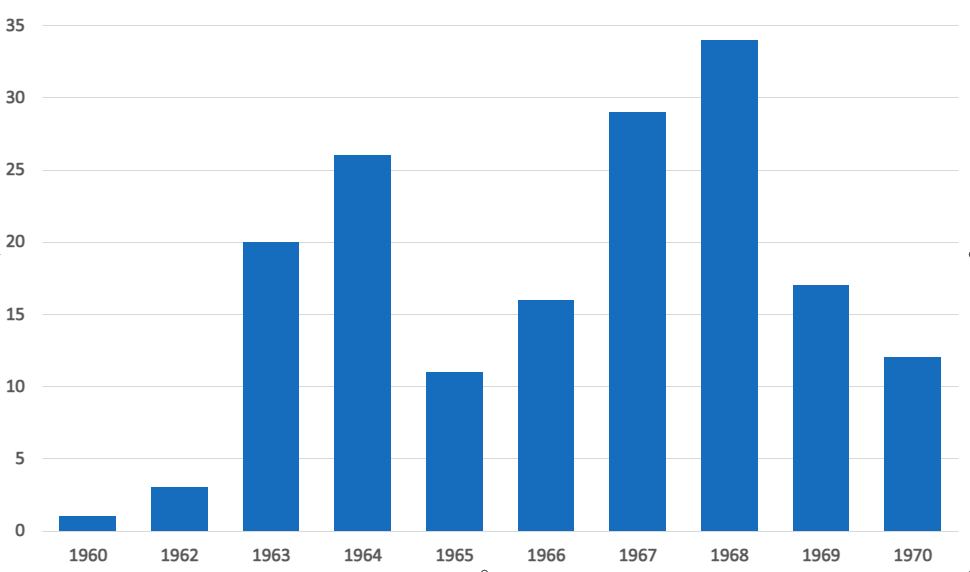
\includegraphics[width=\textwidth]{./chapter/musical_composition/BarChart_number_of_musical_Beatles_by_year_of_publication.png}
	\caption[Гистограмма количества музыкальных композиций The Beatles с 1960 по 1970 годы]
    {Ежегодное количество музыкальных композиций, созданных группой The~Beatles с 1960 по 1970 годы}%
 	\label{fig:ThebeatlesBubbleChart}%
\end{marginfigure}
\end{task}



\newpage
\hfil\pgfornament[width=4cm]{80}\hfil%
%%%%%%%%%%%%%%%%%%%%%%%%%%%%%%%%%%%%%%%%%%%%%%%%%%%%
%%%   radio stations
%%%%%%%%%%%%%%%%%%%%%%%%%%%%%%%%%%%%%%%%%%%%%%%%%%%%
\begin{task}
        \lstset{escapeinside={(*@}{@*)}}
        \sethlcolor{pink}
    \label{answer:radio_stations}

    \AnswerBackref Вопрос на с.~\pageref{question:radio}. 

Вопрос заключался в проблеме вывода результата запроса~\ref{lst:subclasses_of_radio_stations}. Запрос выводил исследуемый объект \wdqName{<<вещательные радиостанции>>}{14350} вместо его подклассов. Проблема заключалась в строке~\lstinline|?subRadio wdt:P279* wd:Q14350|, а именно в символе <<*>>. Это происходит, потому что данный символ объявляет, что нужно учитывать все косвенные подклассы объекта \wdqName{<<вещательные радиостанции>>}{14350} . Если удалить звездочку, то запрос~\ref{lst:subclasses_of_radio_stations} выдаст только непосредственные подклассы \wdqName{<<вещательных радиостанций>>}{14350} без дополнительных уровней вложенности. Исправить ошибку можно путем замены символа <<*>> на символ <<+>>, либо удалением символа <<*>>. Запрос~\ref{lst:subclasses_of_radio_stations} перестанет выводить исследуемый объект и выведет его подклассы.

Ниже представлен исправленный листинг для поиска подклассов~\ref{lst:subclasses_of_radio_stations_fixed} .

\begin{lstlisting}[ 
    language=SPARQL,
    caption={\href{https://w.wiki/9sL8}
                  {Список подклассов радиостанций и размер подклассов}\protect\footnotemark},
    label=lst:subclasses_of_radio_stations_fixed,
    xleftmargin=18pt,
    numbers=left,
    ]
# List of radio subclasses and subclass sizes
SELECT ?subRadio ?subRadioLabel (COUNT(?r) AS ?count) WHERE 
{
  ?subRadio wdt:P279+ wd:Q14350. # subclass of radio station
  ?r wdt:P31 ?subRadio.          # instance of this subclass
  SERVICE wikibase:label { bd:serviceParam wikibase:language "ru,en" }
}
GROUP BY ?subRadio ?subRadioLabel
ORDER BY DESC(?count)
\end{lstlisting}%

\footnotetext{Получено: 22 подкласса радиостанций на 2024 год. 
              Ссылка на SPARQL-запрос: \href{https://w.wiki/9sL8}{https://w.wiki/9sL8}.}
\end{task}

\begin{task}
        \lstset{escapeinside={(*@}{@*)}}
        \sethlcolor{pink}
    \label{answer:radio_stations2}

    \AnswerBackref Вопрос на с.~\pageref{question:radio2}.

В запросах~\ref{lst:radioRussiaUNION} и~\ref{lst:radioRussiaVALUES} мы наблюдали различие в выводе результатов. Ответ кроется в том, что функция UNION и функция VALUES различаются в различии фильтрации данных. Функция UNION не допускает дубликатов, потому что берет одно значение из рассматриваемого свойства (в нашем случае свойство \wdProperty{17}{<<государство>>}). Функция VALUES берет все значения рассматриваемого свойства и выводит их, поэтому в выводе встречаются дубликаты радиостанций. Далее будет приведен пример дубликатов: \wdqName{4729846}{<<Радио-1>>}, \wdqName{3919668}{<<Радио Юность>>}, \wdqName{1589584}{<<Европа плюс>>}. Как мы можем видеть в свойстве \wdProperty{17}{<<государство>>} указаны две страны \wdqName{159}{<<Россия>>} и \wdqName{15180}{<<СССР>>}.

\end{task}
